\documentclass[11pt, letterpaper, oneside]{article}


%\usepackage{microtype}
%\usepackage[utf8]{inputenc}
%\usepackage[T1]{fontenc}
%\usepackage{titlesec}
%\usepackage{graphicx}
%\usepackage{enumitem}
%\usepackage{amsthm}
%%\setlist{nolistsep}
%\usepackage{tikz}
%\graphicspath{{images/}}
%
%\usepackage[utf8]{inputenc}
%\usepackage{amsmath}
%\usepackage{amsfonts}
%\usepackage{amssymb}
%\usepackage[left=2cm,right=2cm,top=2cm,bottom=2cm]{geometry}
%%\usepackage{color}
%\usepackage[usenames,dvipsnames]{xcolor}
%\usepackage{sectsty}
%\usepackage{framed}
%%\usepackage{tikz}
%
%% Font Settings
%\usepackage{avant}
%\usepackage{fourier} 
%\usepackage{charter}
%
%\theoremstyle{definition}
%\newtheorem{definition}{Definition}[section]
%\newtheorem{example}{Ex.}[section]
%\newtheorem{theorem}{Theorem}[section]
%

\usepackage{graphicx}
\graphicspath{{images/}} %image directory

\usepackage{amsmath}
\usepackage{amsfonts}
\usepackage{amssymb}
\usepackage{graphicx}
\usepackage{url}
\usepackage[top=25mm, bottom=25mm, left=30mm, right=25mm]{geometry}
\setlength{\parindent}{0cm} % first para - no indent
\usepackage{titlesec}
\usepackage{setspace}
\usepackage[nottoc]{tocbibind}
\usepackage{listings}
%\usepackage[table]{xcolor}
\usepackage{multirow}
\usepackage{pdflscape}
\usepackage{color}
\usepackage[usenames,dvipsnames]{xcolor}
\usepackage{fancyhdr}
\newtheorem{mydef}{Example}
\titlespacing*{\chapter}{0pt}{0pt}{20pt}
\usepackage{microtype}
\usepackage[toc,page]{appendix}

%\setlist{nolistsep}

% Font settings
\usepackage{avant}
\usepackage{fourier} 
\usepackage{charter}


% Header settings
%\titleformat{\chapter}{\Large\bfseries}{Chapter \thechapter }{14pt}{\Large}
%\titleformat{\chapter}{\Large\bfseries}{\thechapter }{14pt}{\Large}
\titleformat{\section}{\large\bfseries}{{\color{MidnightBlue}\thesection }}{13pt}{\color{MidnightBlue}\large}
\titleformat{\subsection}{\normalsize\bfseries}{ \color{NavyBlue}\thesubsection }{12pt}{\color{NavyBlue}\normalsize}
\titleformat{\paragraph}{\normalsize\bfseries}{ \thesection }{12pt}{\large}

% Itemize - remove exrea linespace
\newlength{\wideitemsep}
\setlength{\wideitemsep}{.5\itemsep}
\addtolength{\wideitemsep}{-7pt}
\let\olditem\item
\renewcommand{\item}{\setlength{\itemsep}{\wideitemsep}\olditem}

% Header and footer
\fancypagestyle{plain}{
\fancyhf{}
\renewcommand{\headrulewidth}{0pt}
\renewcommand{\footrulewidth}{0pt}
\fancyfoot[LE,RO]{\scriptsize{ \thepage} }
%\fancyfoot[RE,LO]{\small ODROID XU4 - Documentation}
%\fancyhead[RO,LE]{\scriptsize{FDCL Document}}
}

\definecolor{maroon}{RGB}{173,34,49}
\definecolor{shadecolor}{RGB}{233,244,255}
\definecolor{exframecolor}{RGB}{255,255,255}
\definecolor{exshadecolor}{RGB}{250,252,252}    
    

\newenvironment{exframe}{
\def\FrameCommand{\fboxrule=\FrameRule\fboxsep=\FrameSep \fcolorbox{exframecolor}{exshadecolor}}
\MakeFramed {\FrameRestore}}
{\endMakeFramed}

% For hyperlinks
\usepackage{hyperref}
\hypersetup{
    colorlinks,
    linkcolor={black!80!black},
    citecolor={blue!50!black},
    urlcolor={blue!80!black}
}

\usepackage{cleveref}  % automatic reference formatting (load AFTER hyperref)
\pagestyle{plain}


\title{Sumo Robot - Report}
\author{Kanishke Gamagedara \\ Kalpesh Patil}

\begin{document}
\thispagestyle{empty}

\begin{center}

%\begin{figure}[h!]
%\begin{center}
%\includegraphics[scale=1]{uni_crest.png}
%\end{center}
%\end{figure}

\vspace*{.5cm}

\title{ \bfseries Sumo Robot \\ Report}
\author{Kalpesh Patil \\ Kanishke Gamagedara\\ {\normalsize kanishkegb@gwu.edu}\\{\normalsize Fall 2016}}

\vspace{10 mm}
 {\bf \color{MidnightBlue} {\Huge Sumo Robot } \vspace{4mm} \hline  \vspace{4mm} {\Huge Report}}\\

\vspace*{6cm}

{\large This is the project report for the robot ``Interpreter'' made for the class MAE 6194 }

\vspace*{5cm}

{\large Kalpesh Patil \\ {\normalsize kalpeshpatil33@gwu.edu }\\ \vspace*{5mm} Kanishke Gamagedara}\\ 
{\normalsize kanishkegb@gwu.edu}\\\vspace*{5mm}{\large Spring 2017}

\vspace*{3cm}

{\LARGE 
The George Washington University}

\end{center}
\newpage



\tableofcontents


% =================================================================================
\newpage
\section{Summary}

\begin{figure}[bth]
	\begin{center}
		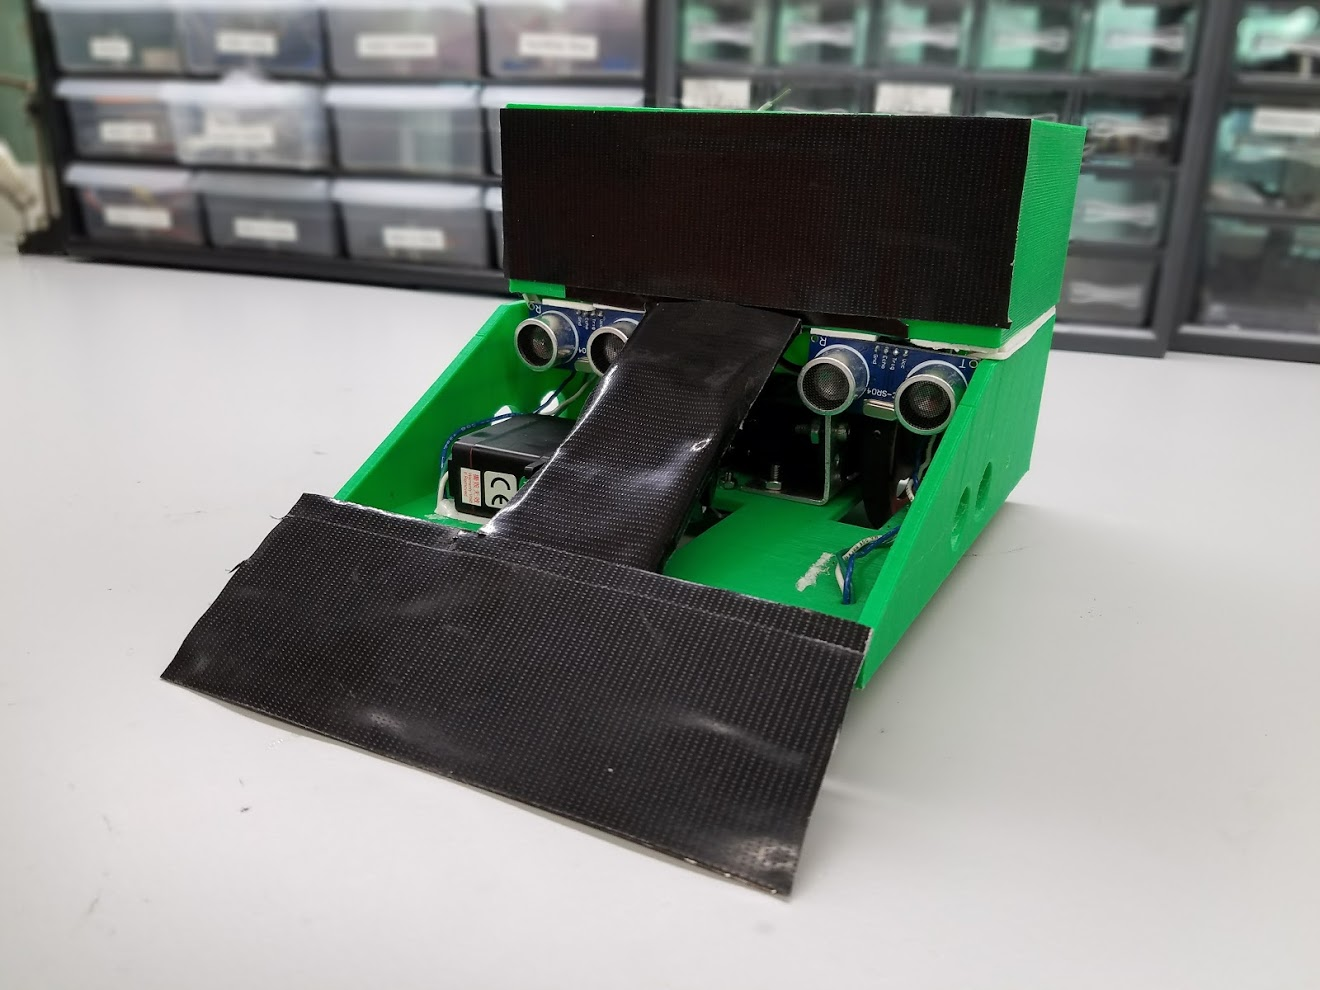
\includegraphics[scale = 0.2]{front.jpg}
		\caption{Interpreter}
		\label{fig:front}
	\end{center}
\end{figure}

We made the ``Interpreter'' for the Sumo Robot Competition, which was held as a part of the course MAE 6194. This robot has an LCD serial monitor, which is operated through XBee, which displays ( or interprets ) everything it does. This lead to the name Interpreter.  The basic functions and features of the robot are listed below.
\begin{itemize}
	\item Finds the opponent using sonar sensors
	\item Detects the line using QTI sensors
	\item If and opponent is detected, accelerates towards it
	\item If the opponent is close enough, raise the flipping shield
	\item Send every task the robot is performing through XBee
	\item Another Arduino board reads the transmitted data via an XBee, and prints to an LCD display
\end{itemize}

This report is organized as follows. First, we will discuss the details on the body structure and the sensors. Then we will be explaining how the attacking mechanism works. Next section is on details of the LCD serial monitor system which is used to continuously monitor and debug the robot. Then we will provide an overview of the overall algorithm which is used to control the robot. Finally the issues we faced and the proposed future developments. The codes are attached in the appendix.


% =================================================================================
\newpage
\section{Physical Structure}

\begin{figure}[bth]
	\begin{center}
		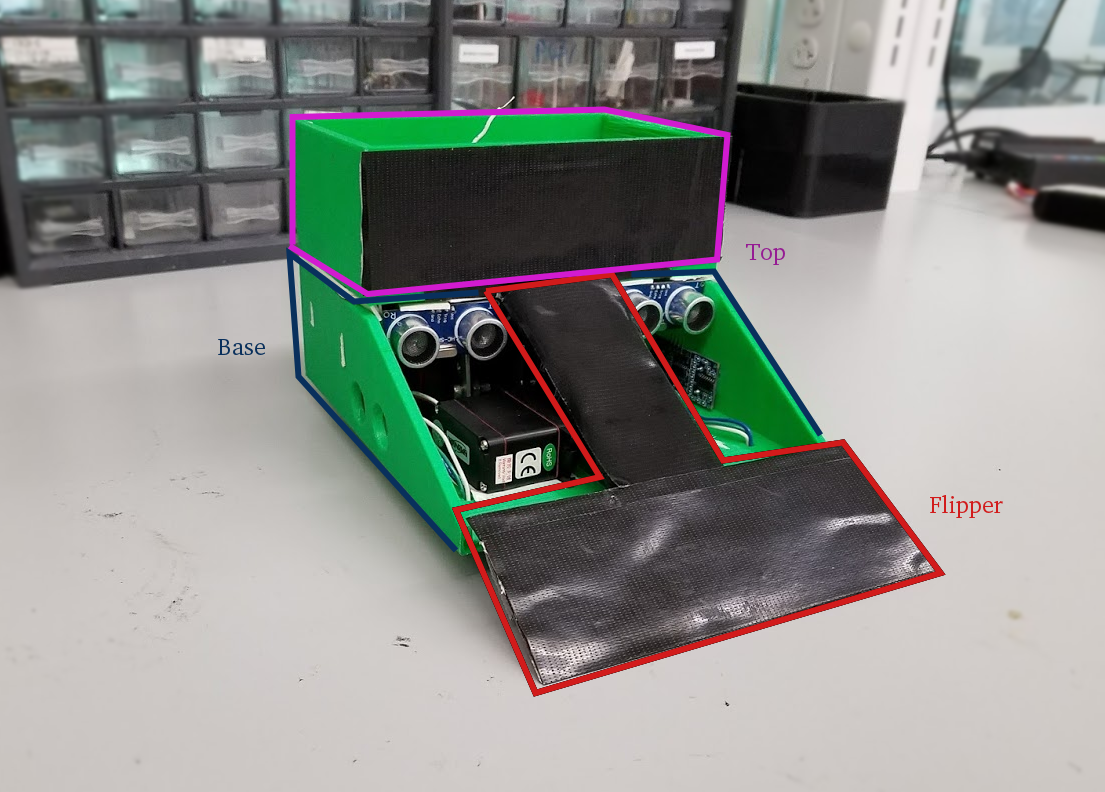
\includegraphics[scale = 0.3]{detailed_structure.png}
		\caption{Structure}
		\label{fig:detailed_structure}
	\end{center}
\end{figure}

In this section, we discuss about the body structure of the robot and the sensors. The robots structure mainly has three parts. 
\begin{enumerate}
	\item Base
	\item Top
	\item Flipper
\end{enumerate}


Base holds all the motors, back and side sonar sensors, and the QTI sensors at the bottom. On top of the Base, we have placed the Top which securely holds the Arduino board, batteries, Xbee unit, and the two front sonar sensors. Flipper is hinged to the front bottom edge of the Top and a servo motor with an arm is placed on the base, directly under the flipper, to activate the attacking mechanism. Top and the Base was 3D-printed and the flipper was cut from a thin wood board and a sheet metal piece at the bottom edge.



% =================================================================================
\newpage
\section{Sensors and Components}
A physical structure of a robot is nothing without sensing or actuation devices. In this section, we describe the sensors and components we used on our robot. \\

\subsection{Line Detection}
The most important objective of a Sumo Robot is to detect the boundary line of the ring. For this, we used QTI sensors by Parallax\footnote{\url{https://www.parallax.com/product/555-27401}}, where QTI stands for Q - charge, T - transfer and, I - infrared. We used three QTI sensors, one in the center and two in the front left and front right.
\begin{figure}[bth]
	\begin{center}
		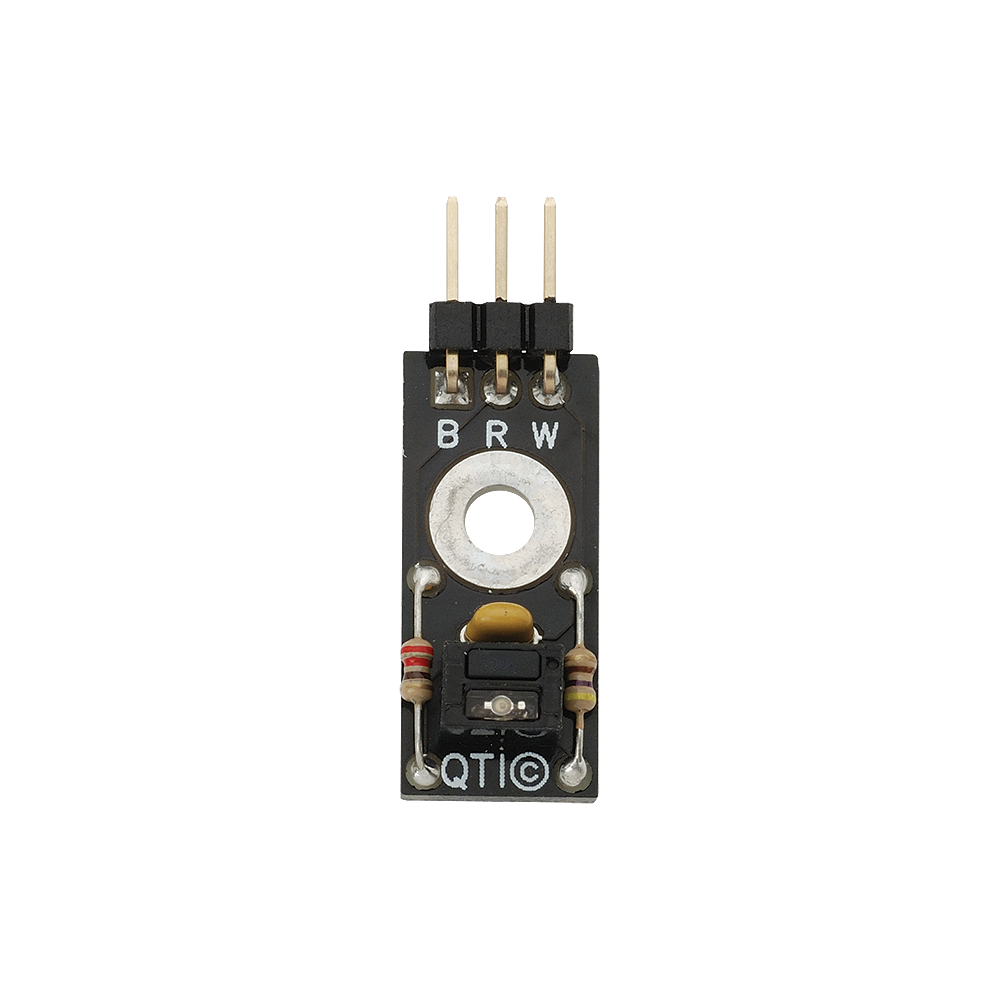
\includegraphics[scale = 0.15]{qti.png}
		\caption{QTI Sensor}
		\label{fig:qti}
	\end{center}
\end{figure}

Referring \cref{fig:qti}, pin W is supplied with 5 V and pin B is connected to the ground. Pin R is the sensor pin. As name implies, the sensor need to be charged. This is done by setting the sensor pin to HIGH during the initialization. In the case of middle QTI sensor, we need to shutdown the robot as soon as it detects the white line. For this, we used interrupts. Example code can be found below.

\begin{verbatim}
void setup() {
    pinMode(MIDDLE_pinQTIsensor, INPUT);  // set sensor pin as an input
    digitalWrite(MIDDLE_pinQTIsensor, HIGH);  // charging phase of the QTI
	
    attachInterrupt(digitalPinToInterrupt(MIDDLE_pinQTIsensor), MIDDLE_whiteLineISR, LOW);
    // attach the interrupt 
 }
 
void MIDDLE_whiteLineISR() {
    goStop();  // stop the robot as soon as middle QTI detects a line
}
\end{verbatim}


\subsection{Sonar Sensors}
The next objective of the robot is to identify the opponent robot. We used five HC-SR04 sonar sensors\footnote{\url{https://goo.gl/ZwPIIL}}. Two sensors were used in the front, and other three were used on left, right and back. The sensor sends a sonar signal and receives it back. The time difference between sending and receiving is used to calculate the distance of and obstacle. The sensor has a range of 2 - 500 cm for obstacle detection.
\begin{figure}[bth]
	\begin{center}
		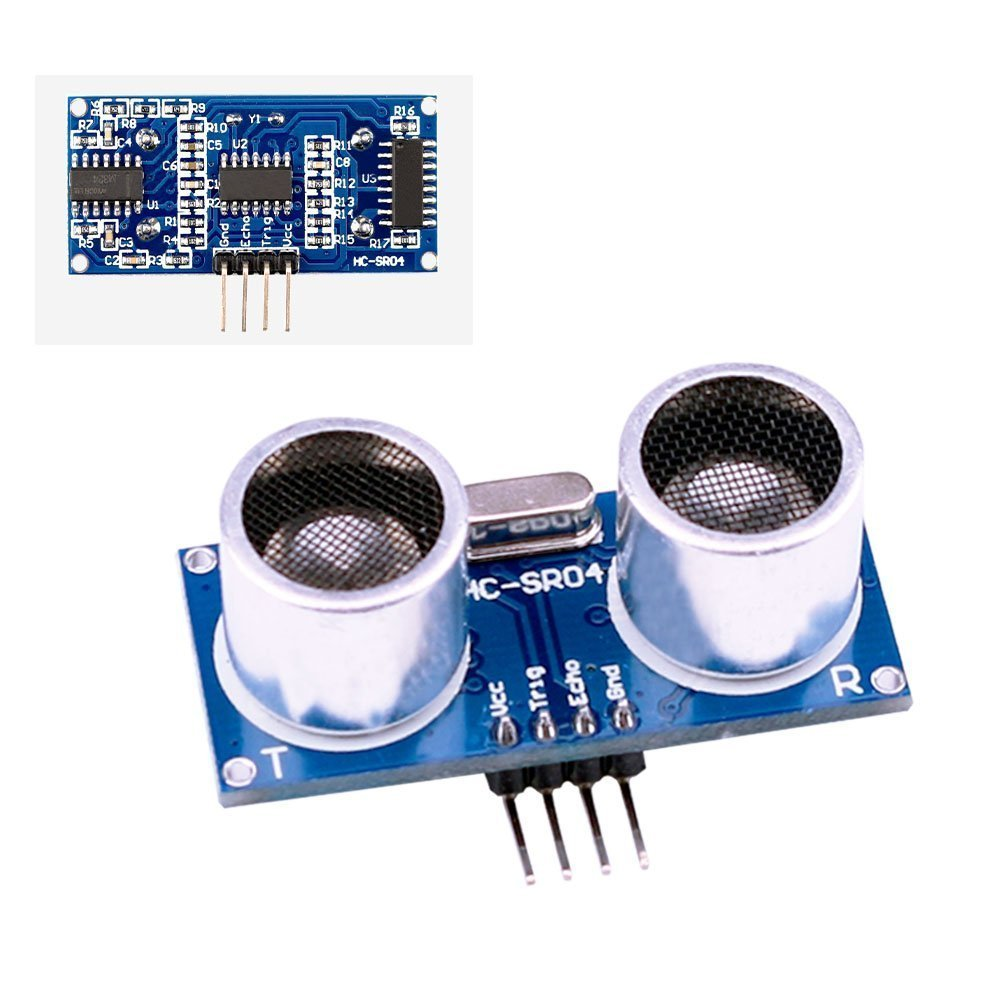
\includegraphics[scale = 0.15]{sonar.jpg}
		\caption{HC-SR04}
		\label{fig:sonar}
	\end{center}
\end{figure}

This sensor has four pins: power, ground, trigger, and echo. Power in is supplied with 5 V. We need to write the pulse to the trigger pin and then read the echo. For this we use built-in Arduino function ``pulseIn''\footnote{\url{https://www.arduino.cc/en/Reference/pulseIn}}. This function returns the time the length of the pulse in microseconds. Since we know that the speed of sound is $340 \; m/s = 0.034 \; cm / \mu s$, we can calculate the distance to the obstacle.

\begin{verbatim}
int FRONT_distance = 0  // initialize the distance to an obstacle facing front 
                        // sensor as a global variable

void FRONT_HC() {
    // writes the pulse
    digitalWrite(FRONT_trigPin, LOW);
    digitalWrite(FRONT_trigPin, HIGH);
    delay(100);                      
    digitalWrite(FRONT_trigPin, LOW);
    
    FRONT_duration = pulseIn(FRONT_echoPin, HIGH);  // read the echo
    FRONT_distance = (FRONT_duration / 2) * 0.034;  // calculate the distance
}

void loop {
    FRONT_HC();  // call the front sonar function
}
\end{verbatim}


\subsection{Motors}
Motors are the actuators of our robot. We used three motors: two for the motion of the robot and one for the attacking mechanism. For the wheel motors, we use Parallax continuous rotation servo motors\footnote{\url{https://www.parallax.com/product/900-00008}}. Each of the motors has a power pin ( 5 V ), ground pin, and a servo pin. In this section we mainly focus on wheel motors. The motor we used for the attacking mechanism is described in \cref{sec:attacking}.

\begin{figure}[bth]
	\begin{center}
		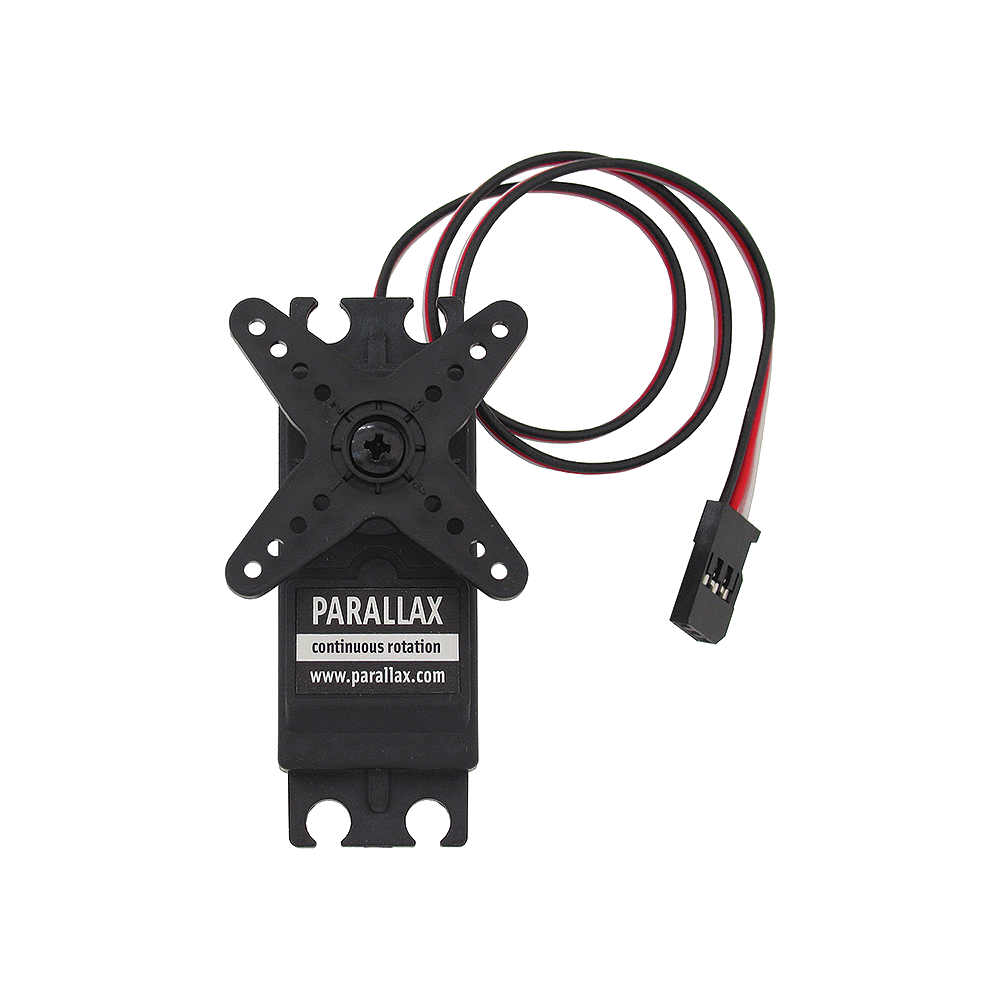
\includegraphics[scale = 0.2]{servo.png}
		\caption{ Parallax continuous rotation servo motor}
		\label{fig:servo}
	\end{center}
\end{figure}

First thing you have to do with the servo is to calibration. For example, servo motor is supposed to stop when the servo pin is written 90. But, there might be cases where the motor might not be 100\% stopped when 90 is written to the servo pin. To calibrate, we have to write 90 to servo and rotate the small screw until the motor is completely stopped. We have two servo motors facing opposite sides. The list of servo pin values that need to written to each motor is given in \cref{tab:servo}

\begin{table}[tbh]
	\caption{Servo pin values to be written for each operation}
	\label{tab:servo}
	\begin{center}
		\begin{tabular}{|l|c|c|}
			\hline
			Operation 	& 	Left motor	&	Right motor \\ 	\hline 
			Forward 	& 	0 			&	190 		\\
			Backward 	& 	190			&	0 			\\ 
			Stop		&	90 			&	90 			\\
			Left rotate	&	0			&	0			\\
			Right rotate&	190			&	190			\\	\hline 
		\end{tabular}
	\end{center}
\end{table} 

Further, depending on the time period you write these values, we can determine the angle of rotation. If you left rotate for $200\;ms$ and $400 \;ms$, robot will turn 90 and 180 degrees respectively.\\

Belowgit at snippet gives a basic idea on this.
\begin{verbatim}
// define servo pins as global variables
#define LEFT_servo = 9 
#define RIGHT_servo = 10

void setup() {
    // attach the servos to servo object
    leftServo.attach(LEFT_servo); 
    rightServo.attach(RIGHT_servo); 
}

void goRight() {
    leftServo.write(190);
    rightServo.write(190);
}

void goStop() {
    leftServo.write(90);
    rightServo.write(90);
}

void loop() {
    // rotate 90 degrees right
    goRight();
    delay(200);
    
    // stop
    goStop();
    
    // rotate 180 degrees right
    goRight();
    delay(200);
}
\end{verbatim}



% =================================================================================
\newpage
\section{Attacking Mechanism} \label{sec:attacking}
In this section, we explain details about the attacking mechanism installed in our robot. Our mechanism is a simpler flipper in front of the robot. The flipper as described in \cref{fig:front} is in rest position when it is in non-attacking mode. The front edge is touching the ground so that the opponent might ride up the top surface of the flipper (refer \cref{fig:attacking_low} ). 

\begin{figure}[bth]
	\begin{center}
		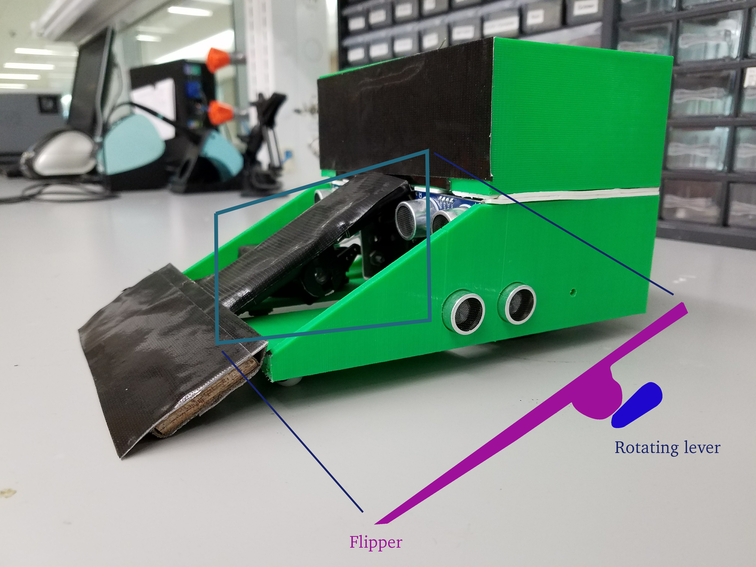
\includegraphics[scale = 0.36]{attacking_low.png}
		\caption{ Flipper in resting position}
		\label{fig:attacking_low}
	\end{center}
\end{figure}


As soon as the front sonar sensors detect an object closer than $8\;cm$, the attack servo motor starts rotating rising the flipper (refer \cref{fig:attacking_high}).

\begin{figure}[bth]
	\begin{center}
		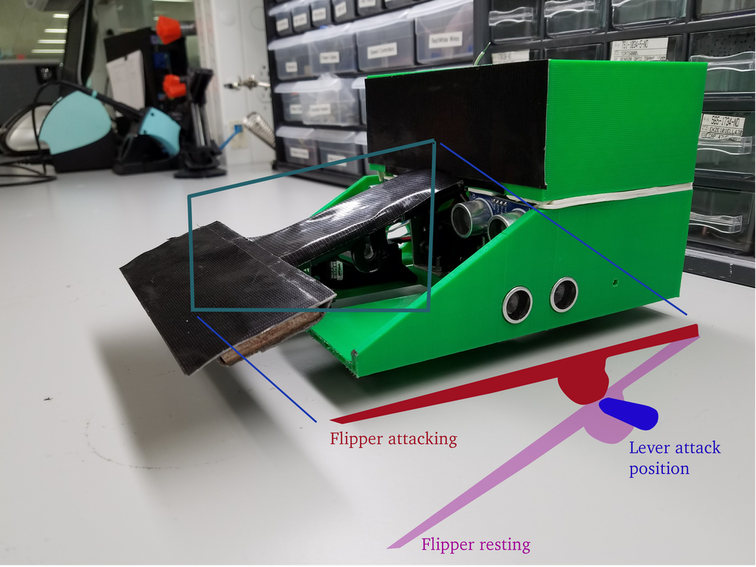
\includegraphics[scale = 0.36]{attacking_high.png}
		\caption{ Flipper in action}
		\label{fig:attacking_high}
	\end{center}
\end{figure}


% =================================================================================
\newpage
\section{Wireless LCD Serial Monitor}
Display system is our innovation part and this subsystem gives our robot its name ``Interpreter''. Arduino board needs to be programmed the way we need the robot to work. But we might not be able to write a code such that the robot does exactly what we need it to do, in the first time. We had to do change parameters, add or delete lines, or change the whole sections of the code multiple times until the robot does exactly what we want it to do. \\

While we were debugging the code, we faced instances where we wanted see which function the robot is executing when it performs an unnecessary action. First option is to use the serial monitor in Arduino IDE. But, it requires a cable connection between Arduino board and a laptop. This is not convenient since you have to run with the robot carrying your laptop. Instead, we decided to develop a wireless data transmission system using XBees and an LCD display system to act as a serial monitor.\\

\begin{figure}[bth]
	\begin{center}
		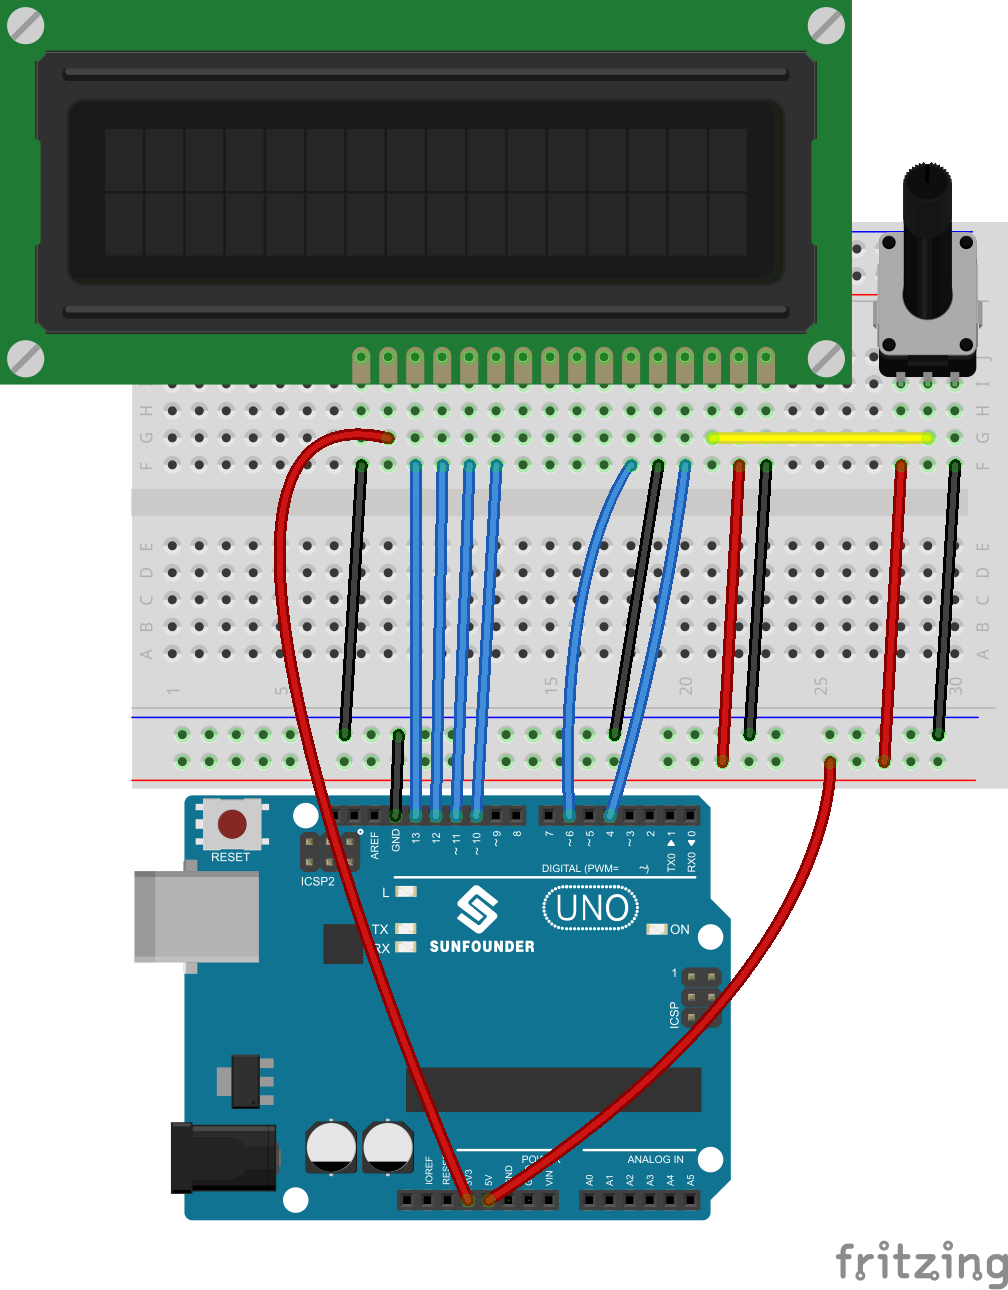
\includegraphics[scale = 0.7]{lcd_wiring.png}
		\caption{LCD wiring diagram}
		\label{fig:lcd_wiring}
	\end{center}
\end{figure}

Our code inside the robot is a collection of function and we call each function in the main loop. Each function is assigned with an integer. We connected one Xbee for a Serial port in the robot Arduino. When a function is called, the integer assigned with the function is sent to XBee. We have another XBee, where the paired other XBee is attached. An LCD display also is attached to this Arduino board. The program inside this Arduino reads from XBee and prints to the LCD screen.\\


\Cref{fig:lcd_wiring} shows the wiring diagram for the LCD\footnote{\url{https://www.sunfounder.com/media/wysiwyg/swatches/super-kit-v2-for-Arduino/8_LCD1602/fri_lcd.png}}. Below snippet shows how our system runs on the robots Arduino board. This keeps writing integer 6 to the XBee.
\newpage
\begin{verbatim}
int_lcd = 0  \\ integer for LCD system

void setup() {
    Serial.begin(115200);  \\ initialize XBee serial port
}

void goAttack() {
    Serial.println("Attack");
    attackServo.write(0);
    int_lcd = 6;
}

void loop() {
    goAttack()
}
\end{verbatim}


Second Arduino board's code will read this value and print respective string to the LCD display (refer \cref{fig:lcd}). This part is hard to show as a snippet. So please refer Appendix 2.


\begin{figure}[bth]
	\begin{center}
		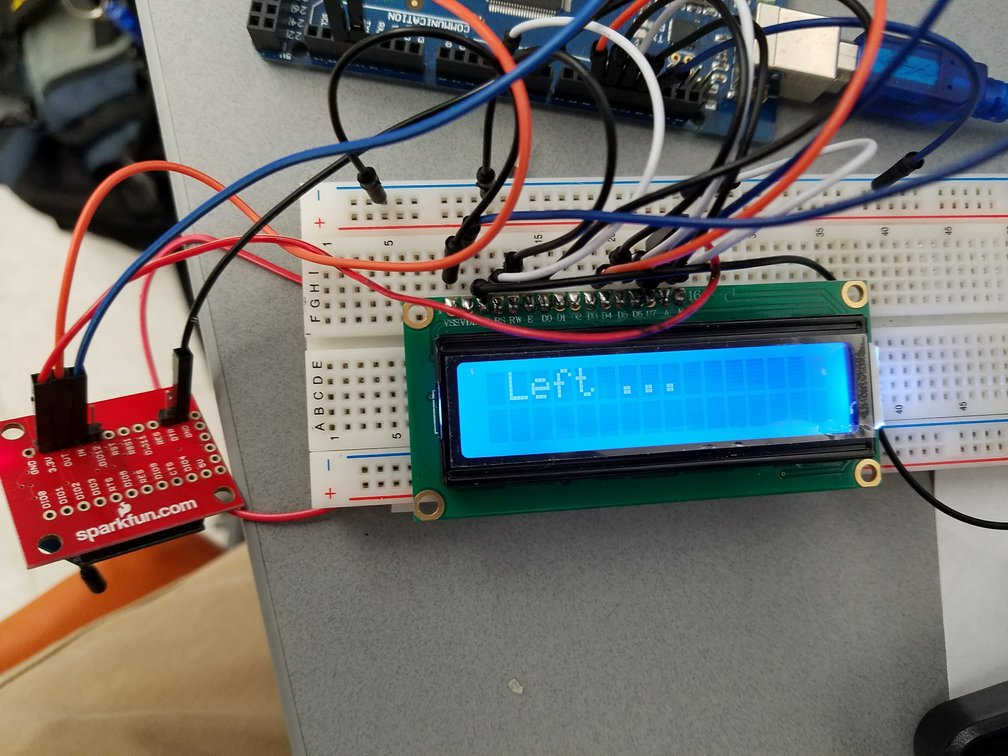
\includegraphics[scale = 0.36]{lcd.jpg}
		\caption{LCD serial monitor}
		\label{fig:lcd}
	\end{center}
\end{figure}


% =================================================================================
\newpage
\section{Algorithm}
\begin{figure}[h!]
	\begin{center}
		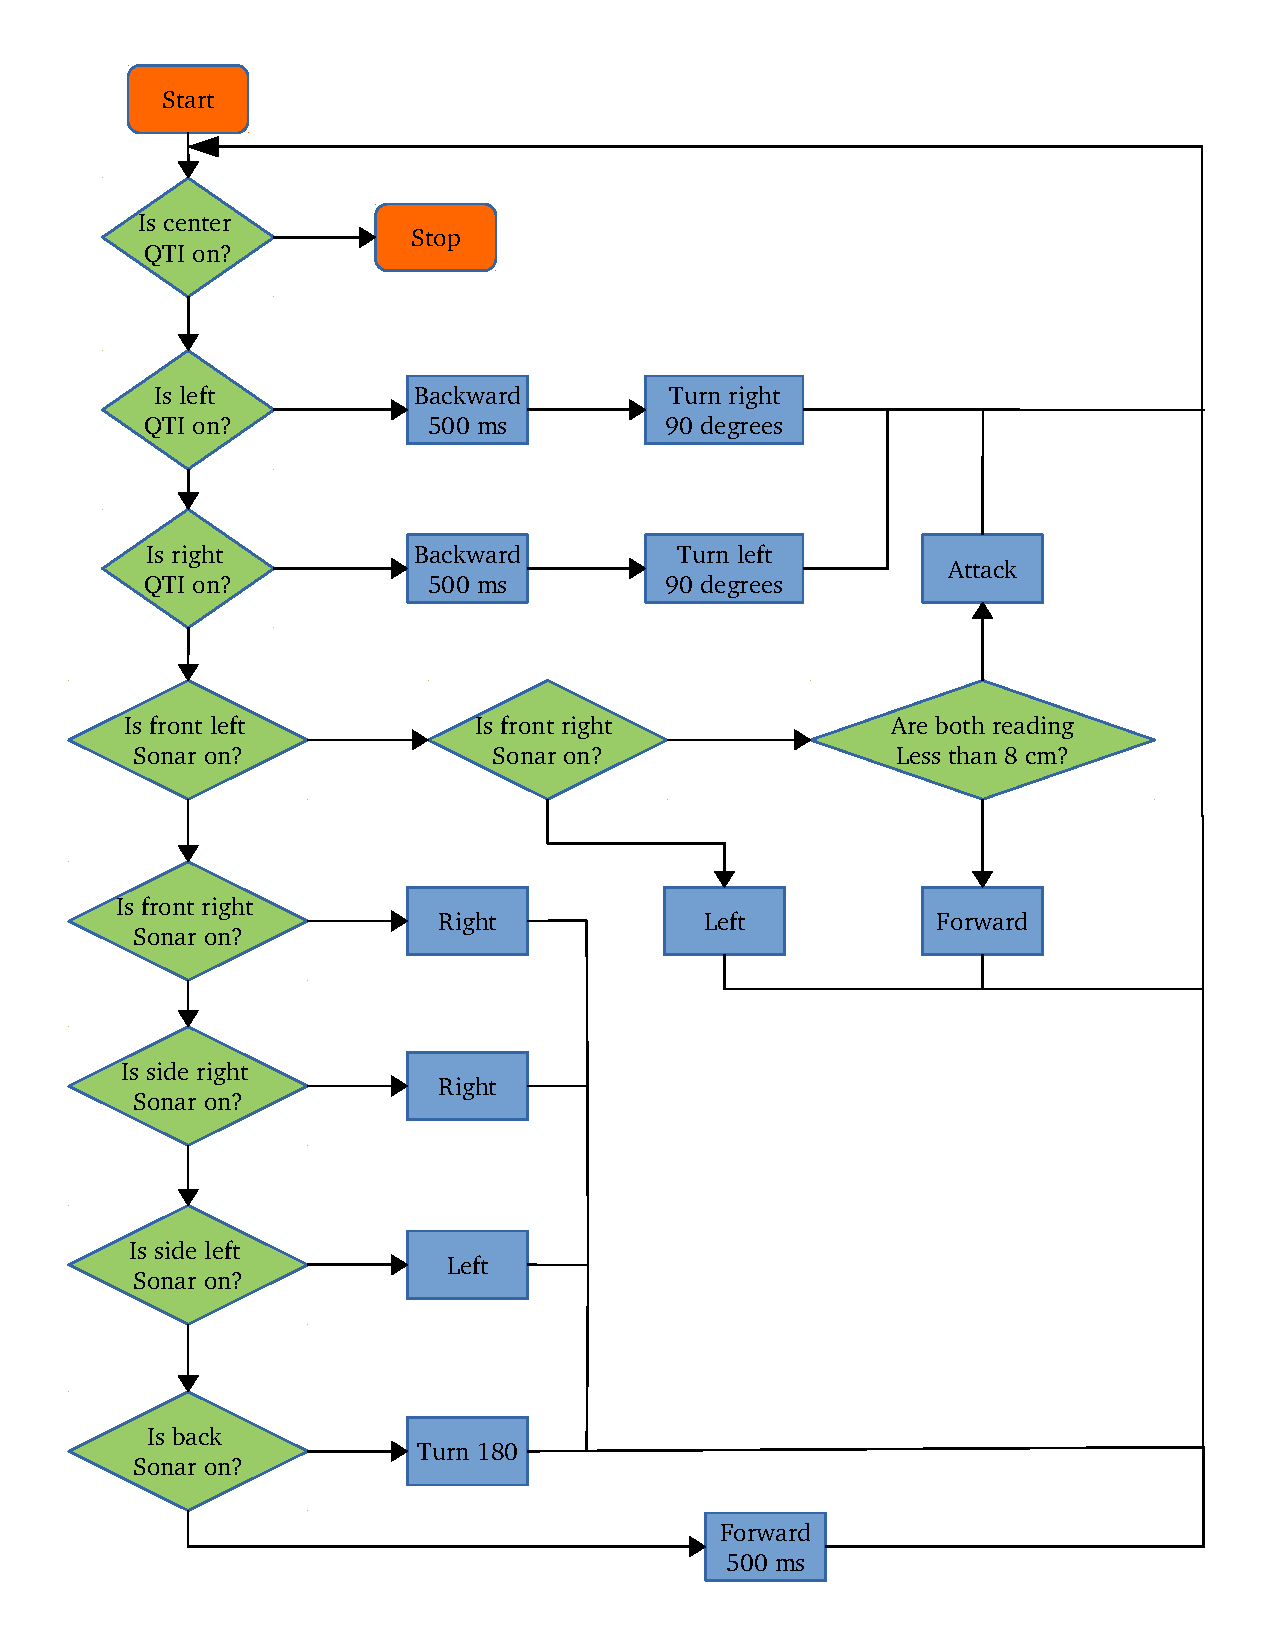
\includegraphics[scale = 0.7]{flowchart.pdf}
		% \caption{LCD serial monitor}
		\label{fig:flowchart}
	\end{center}
\end{figure}

Please note that in this diagram, all the downwards arrows represent ``No'' and every other arrow represent ``Yes''.
% =================================================================================
\newpage
\section{Future Developments}

We faced few problems while working on this. One was the wheel we used. We used a wheel with a thin rubber tire. During the competition, the rubber part of the wheel worn out due to friction. This lost the grip on our robot while pushing the other robots. One major future development will be getting thicker tires.\\

Further, we suggest using two more QTI sensors on the back of the chassis. It will detect if the robot is being pushed backwards and we can program robot to move sideways to avoid being pushed all the way out.\\

Another major improvement will be adding optical sensors/ IR sensors as a secondary opponent recognition sensor. Some opponents were using sonar absorbing/ non-reflecting materials to cover their robots. Having this secondary system will avoid such situations.\\

Unfortunately, our attacking mechanism stopped working during the competition due to loose connection. We could not figure it out during the competition. Our last future improvement is to have a proper printed PCB instead of using jumper cables.

% =================================================================================
\newpage
\section{List of Components}
\begin{table}[tbh]
	\label{tab:components}
	\begin{center}
		\begin{tabular}{|l|c|r|}
			\hline
			Component 		& 	No. of units	&	Unit price 	\\ 	\hline 
			Wheels	 		& 	2 				&	\$3.50 		\\
			Attack servo	&	1 				&	\$8.99 		\\
			QTI				&	1				&	\$9.99		\\
			Sonar sensors	&	1 set of 5		&	\$15.99		\\	\hline 
		\end{tabular}
	\end{center}
\end{table} 

% =================================================================================
\newpage
\section{Appendix 1: Sumo Robot Code}
\begin{verbatim}
int int_lcd = 0;
int int_lcd_prev = 0;
int t_delay = 200;

#define LEDPIN 22  // LED

// Wheel Variables
#include <Servo.h>
Servo leftServo;
Servo rightServo;
Servo attackServo;
#define LEFT_servo 4
#define RIGHT_servo 5
#define ATTACK_servo 7

// Sonar distances
#define HCdistance 50
#define AttackHCdistance 8

// QTI MIDDLE Variable
volatile int MIDDLE_whiteLine = 1;
int MIDDLE_sensorVal;
#define MIDDLE_pinQTIsensor 2

// QTI LEFT Variable
volatile int LEFT_whiteLine;
int LEFT_sensorVal;
#define LEFT_pinQTIsensor 6

// QTI RIGHT Variable
volatile int RIGHT_whiteLine;
int RIGHT_sensorVal;
#define RIGHT_pinQTIsensor 3

// HC-SR04 FRONT LEFT Variable
#define FRONT_LEFT_trigPin 27
#define FRONT_LEFT_echoPin 28
long FRONT_LEFT_duration, FRONT_LEFT_distance;

// HC-SR04 FRONT RIGHT Variable
#define FRONT_RIGHT_trigPin 29
#define FRONT_RIGHT_echoPin 30
long FRONT_RIGHT_duration, FRONT_RIGHT_distance;

// HC-SR04 BACK Variable
#define BACK_trigPin 9
#define BACK_echoPin 8
long BACK_duration, BACK_distance;

// HC-SR04 LEFT Variable
#define LEFT_trigPin 11
#define LEFT_echoPin 10
long LEFT_duration, LEFT_distance;

// HC-SR04 RIGHT Variable
#define RIGHT_trigPin 13
#define RIGHT_echoPin 12
long RIGHT_duration, RIGHT_distance;


void goForward() {
  // moves robot forward
  leftServo.write(0);
  rightServo.write(190);
  int_lcd = 1;
}

void goBackward() {
  // moves robot backward
  leftServo.write(190);
  rightServo.write(0);
  int_lcd = 2;
}

void goLeft() {
  // moves robot left
  leftServo.write(0);
  rightServo.write(0);
  int_lcd = 3;
}

void goRight() {
  // moves robot right
  leftServo.write(190);
  rightServo.write(190);
  int_lcd = 4;
}

void goStop() {
  // stops robot
  digitalWrite(22, HIGH);
  leftServo.write(90);
  rightServo.write(90);
  attackServo.write(90);
  int_lcd = 5;
}

void goAttack() {
  // starts flipping
  attackServo.write(0);
  int_lcd = 6;
}

void goU() {
  // turn 180
  leftServo.write(0);
  rightServo.write(0);
  int_lcd = 7;
}

void FRONT_LEFT_HC() {
  digitalWrite(FRONT_LEFT_trigPin, LOW);
  digitalWrite(FRONT_LEFT_trigPin, HIGH);
  delay(100);
  digitalWrite(FRONT_LEFT_trigPin, LOW);
  FRONT_LEFT_duration = pulseIn(FRONT_LEFT_echoPin, HIGH);
  FRONT_LEFT_distance = (FRONT_LEFT_duration / 2) * 0.034;
}

void FRONT_RIGHT_HC() {
  digitalWrite(FRONT_RIGHT_trigPin, LOW);
  digitalWrite(FRONT_RIGHT_trigPin, HIGH);
  delay(100);
  digitalWrite(FRONT_RIGHT_trigPin, LOW);
  FRONT_RIGHT_duration = pulseIn(FRONT_RIGHT_echoPin, HIGH);
  FRONT_RIGHT_distance = (FRONT_RIGHT_duration / 2) * 0.034;
}

void BACK_HC() {
  digitalWrite(BACK_trigPin, LOW);
  digitalWrite(BACK_trigPin, HIGH);
  digitalWrite(BACK_trigPin, LOW);
  BACK_duration = pulseIn(BACK_echoPin, HIGH);
  BACK_distance = (BACK_duration / 2) * 0.034;
}

void LEFT_HC() {
  digitalWrite(LEFT_trigPin, LOW);
  digitalWrite(LEFT_trigPin, HIGH);
  digitalWrite(LEFT_trigPin, LOW);
  LEFT_duration = pulseIn(LEFT_echoPin, HIGH);
  LEFT_distance = (LEFT_duration / 2) * 0.034;
}

void RIGHT_HC() {
  digitalWrite(RIGHT_trigPin, LOW);
  digitalWrite(RIGHT_trigPin, HIGH);
  digitalWrite(RIGHT_trigPin, LOW);
  RIGHT_duration = pulseIn(RIGHT_echoPin, HIGH);
  RIGHT_distance = (RIGHT_duration / 2) * 0.034;
}

void setup() {

  Serial.begin(115200);  // XBee serial port
  pinMode(LEDPIN, OUTPUT);  // LED is off at the beginning

  // attach sevos
  leftServo.attach(LEFT_servo);
  rightServo.attach(RIGHT_servo);
  attackServo.attach(ATTACK_servo);

  // initialize QTIs
  pinMode(LEFT_pinQTIsensor, INPUT);
  pinMode(MIDDLE_pinQTIsensor, INPUT);
  pinMode(RIGHT_pinQTIsensor, INPUT);

  digitalWrite(LEFT_pinQTIsensor, HIGH);
  digitalWrite(MIDDLE_pinQTIsensor, HIGH);
  digitalWrite(RIGHT_pinQTIsensor, HIGH);

  // attach interrupt
  attachInterrupt(digitalPinToInterrupt(MIDDLE_pinQTIsensor), MIDDLE_whiteLineISR, LOW);
  interrupts(); // enable interrupts

  // configure sonar sensor pins
  pinMode(FRONT_LEFT_trigPin, OUTPUT);
  pinMode(FRONT_LEFT_echoPin, INPUT);
  pinMode(FRONT_RIGHT_trigPin, OUTPUT);
  pinMode(FRONT_RIGHT_echoPin, INPUT);
  pinMode(BACK_trigPin, OUTPUT);
  pinMode(BACK_echoPin, INPUT);
  pinMode(LEFT_trigPin, OUTPUT);
  pinMode(LEFT_echoPin, INPUT);
  pinMode(RIGHT_trigPin, OUTPUT);
  pinMode(RIGHT_echoPin, INPUT);

  // do not move at the beginning
  goStop();
  delay(500);
}

// interrupt for the middle QTI
void MIDDLE_whiteLineISR() {
  goStop();
  MIDDLE_whiteLine = 0;
  int_lcd = 10;
}

void loop() {
  // read from sonar sensors
  FRONT_LEFT_HC();
  FRONT_RIGHT_HC();
  LEFT_HC();
  RIGHT_HC();
  BACK_HC();

  // read QTI sensors
  LEFT_sensorVal = digitalRead(LEFT_pinQTIsensor);
  RIGHT_sensorVal = digitalRead(RIGHT_pinQTIsensor);

  // if front right QTI is on
  if (  RIGHT_sensorVal == 0 ) {
    goBackward();
    delay(500);
    goLeft();
    delay(t_delay);
  }

  // if front left QTI is on
  if (  LEFT_sensorVal == 0 ) {
    goBackward();
    delay(500);
    goRight();
    delay(t_delay);
  }

  // do if middle QTI is not detecting line
  if (MIDDLE_whiteLine == 1) {

    // if opponent is closer, attack
    if (FRONT_LEFT_distance < AttackHCdistance && FRONT_RIGHT_distance < AttackHCdistance ) {
      goAttack();
      delay(t_delay);
    }

    // if opponent is forward, go push
    if (FRONT_LEFT_distance < HCdistance && FRONT_RIGHT_distance < HCdistance) {
      goForward();
      delay(t_delay);
    }

    // if opponent is forward left, go left
    if (FRONT_LEFT_distance < HCdistance && FRONT_RIGHT_distance > HCdistance) {
      goForward();
      delay(t_delay);
    }

    // if opponent is forward right, go right
    if (FRONT_LEFT_distance > HCdistance && FRONT_RIGHT_distance < HCdistance) {
      goForward();
      delay(t_delay);
    }

    // if opponent is on left, go left
    if (LEFT_distance < HCdistance ) {
      goLeft();
      delay(t_delay);
    }

    // if opponent is on right, go right
    if (RIGHT_distance < HCdistance ) {
      goRight();
      delay(t_delay);
    }

    // if opponent is on back, rotate 180
    if (BACK_distance < HCdistance) {
      goU();
      delay(2 * t_delay);
    }
  }
  else {
    goStop();
    digitalWrite(LEDPIN, HIGH);
    while (1);
  }

  // update XBee only if LCD int is changed
  if (int_lcd_prev != int_lcd) {
    Serial.println(int_lcd_prev);
  }
  int_lcd_prev = int_lcd;
}
\end{verbatim}


% =================================================================================
\newpage
\section{Appendix 2: Wireless LCD Serial Monitor Code} \label{sec:lcd_code}
\begin{verbatim}
#include <LiquidCrystal.h>                  // include the library code

char array1[] = " Bot Info               "; // welcome string

int delay_t = 200; //the value of delay delay_tef
int positionCounter1 = 0; // for left moving animation

// initialize the library with the numbers of the interface pins
LiquidCrystal lcd(4, 6, 10, 11, 12, 13);

void setup() {
  Serial1.begin(115200);  // Xbee
  lcd.begin(16, 2);       // set up the LCD's number of columns and rows:
  lcd.clear();            // clear the LCD
  lcd.setCursor(15, 0);   // set the cursor to column 15, line 0

  // flush the buffer
  while (Serial1.available() > 0)
    Serial1.read();

  // print welcome string
  positionCounter1 = 0;
  while (positionCounter1 < 15) {
    lcd.scrollDisplayLeft();
    lcd.print(array1[positionCounter1]);
    delay(delay_t);
    positionCounter1++;
  }
}



void loop() {
  String in;
  if (Serial1.available() > 0) {
    // read the string from XBee 
    in = Serial1.readStringUntil('\n');
  }

  // convert the String to Int
  int in_int = in.toInt();

  lcd.setCursor(0, 1);
  lcd.clear();

  // print the respective string to LCD
  switch (in_int) {
    case 1:
      Serial.println(in_int);
      lcd.print(" Robot in front      ");
      break;
    case 2:
      lcd.print(" Go back ..      ");
      break;
    case 3:
      lcd.print(" Left ...      ");
      break;
    case 4:
      lcd.print(" Right ...      ");
      break;
    case 5:
      lcd.print(" Stop !      ");
      break;
    case 6:
      lcd.print("Attack      ");
      break;
    case 7:
      lcd.print(" Rotate 180   ");
      break;
    case 10:
      lcd.print("  Middle QTI int.  ");
      break;
    default:
      break;
  }

  //  lcd.print(in_int);
  delay(1000);

  // flush the buffer
  while (Serial1.available() > 0)
    Serial1.read();
}
\end{verbatim}

\end{document}